% begin module horizontal-asymptote-def
\begin{frame}
\begin{definition}[Horizontal Asymptote]
The line $y = L$ is called a horizontal asymptote of $f$ if either
\[
\lim_{x\to \infty}f(x) = L \qquad \text{ or } \qquad \lim_{x\to - \infty} f(x) = L.
\]
\end{definition}
\begin{itemize}
\item<2->  For example, $y = 1$ is a horizontal asymptote for $f(x) = \frac{x^2-1}{x^2+1}$.%
\item<3->  Can a function have two horizontal asymptotes?  \alert<handout:0| 4>{\uncover<4->{Yes.}}%
\end{itemize}
\uncover<4->{%
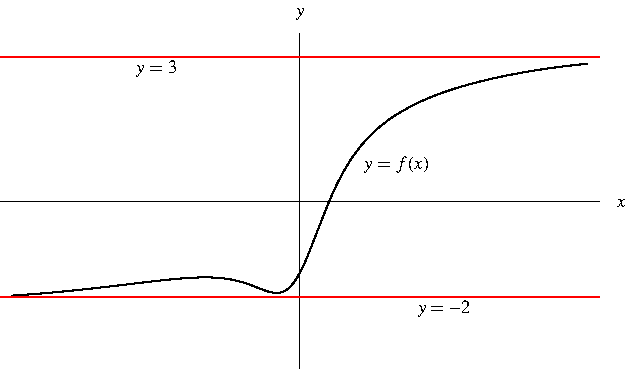
\includegraphics[width=8cm]{curve-sketching/pictures/04-04-twoasymptote.pdf}%
}%
\end{frame}
% end module horizontal-asymptote-def
